\documentclass[12pt]{article}
\usepackage[utf8]{inputenc}

\usepackage{lmodern}

\usepackage{enumitem}
\usepackage[margin=2cm]{geometry}

\usepackage{amsmath, amsfonts, amssymb}
\usepackage{graphicx}
%\usepackage{subfigure}
\usepackage{tikz}
\usepackage{pgfplots}
\usepackage{multicol}

\usepackage{comment}
\usepackage{url}
\usepackage{calc}
\usepackage{subcaption}
\usepackage[indent=0pt]{parskip}
\usepackage{animate}

\usepackage{array}
\usepackage{blkarray,booktabs, bigstrut}
\usepackage{bigints}

\pgfplotsset{compat=1.16}

% MATH commands
\newcommand{\ga}{\left\langle}
\newcommand{\da}{\right\rangle}
\newcommand{\oa}{\left\lbrace}
\newcommand{\fa}{\right\rbrace}
\newcommand{\oc}{\left[}
\newcommand{\fc}{\right]}
\newcommand{\op}{\left(}
\newcommand{\fp}{\right)}

\newcommand{\bi}{\mathbf{i}}
\newcommand{\bj}{\mathbf{j}}
\newcommand{\bk}{\mathbf{k}}
\newcommand{\bF}{\mathbf{F}}

\newcommand{\mR}{\mathbb{R}}

\newcommand{\ra}{\rightarrow}
\newcommand{\Ra}{\Rightarrow}

\newcommand{\sech}{\mathrm{sech}\,}
\newcommand{\csch}{\mathrm{csch}\,}
\newcommand{\curl}{\mathrm{curl}\,}
\newcommand{\dive}{\mathrm{div}\,}

\newcommand{\ve}{\varepsilon}
\newcommand{\spc}{\vspace*{0.5cm}}

\DeclareMathOperator{\Ran}{Ran}
\DeclareMathOperator{\Dom}{Dom}

\newcommand{\exo}[1]{\noindent\textcolor{red}{\fbox{\textbf{Problem {#1}}}\hrulefill}\\}
\newcommand{\qu}[4]{\noindent\textcolor{#4}{\fbox{\textbf{Section {#1} | Problem {#2}}} \hrulefill{{\fbox{\textbf{{#3} Points}}}}\\}}

\newcommand{\semester}{Spring 2023}

\newcommand{\CVup}{%

\begin{tikzpicture}
\draw[black, <->, >=latex] (-0.33, 0.5) .. controls (-0.125, 0) and (0.125, 0) .. (0.33, 0.5);
\end{tikzpicture}}

\newcommand{\CVupInc}{%
\begin{tikzpicture}
\draw[black, ->, >=latex] (0,0) .. controls (0.2, 0) and (0.4, 0.2) .. (0.5, 0.5);
\end{tikzpicture}}

\newcommand{\CVupDec}{%
\begin{tikzpicture}[rotate=270]
\draw[black, ->, >=latex] (0,0) .. controls (0.2, 0) and (0.4, 0.2) .. (0.5, 0.5);
\end{tikzpicture}}

\newcommand{\CVdown}{%
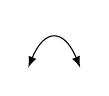
\begin{tikzpicture}
\draw[black, <->, >=latex] (-0.33, -0.5) .. controls (-0.125, 0) and (0.125, 0) .. (0.33, -0.5);
\end{tikzpicture}}

\newcommand{\CVdownInc}{%
\begin{tikzpicture}
\draw[black, ->, >=latex] (-0.5, -0.5) .. controls (-0.5, -0.3) and (-0.5, -0.1) .. (0,0);
\end{tikzpicture}}

\newcommand{\CVdownDec}{%
\begin{tikzpicture}[rotate=-90]
\draw[black, ->, >=latex] (-0.5, -0.5) .. controls (-0.5, -0.3) and (-0.5, -0.1) .. (0,0);
\end{tikzpicture}}

\begin{document}
	\noindent \hrulefill \\
	MATH-241 \hfill Pierre-Olivier Paris{\'e}\\
	Solutions Section 1-8 \hfill \semester \\\vspace*{-1cm}
	
	\noindent\hrulefill
	
	\spc
	
	\exo{18}
	\\
	As $x \ra -2^-$, we have $f(x) \ra -\infty$ and as $x \ra -2^+$, we have $f(x) \ra \infty$. So we have an infinite discontinuity. 
	
	\spc
	
	\exo{36}
	\\
	The function $x + \sin x$ is continuous because it is the sum of two continuous functions. Now, $\sin x$ is continuous and therefore the composition $\sin (x + \sin x )$ is continuous. In particular, the function $x \mapsto \sin (x + \sin x)$ is continuous at $x = \pi$. Using the continuity, this means that
		\begin{align*}
		\lim_{x \ra \pi} \sin (x + \sin x ) = \sin (\pi + \sin \pi ) = \sin (\pi + 0) = 0 .
		\end{align*}
		
	\spc
	
	\exo{56}
	\\
	Let $f(x) = \sin x - x^2 + x$. We have $a = 1$ and $b = 2$. 
	
	We will verify if the hypothesis of the Intermediate Value Theorem are verified. 
		\begin{itemize}
		\item The function $f$ is a sum of continuous function on all of $(-\infty , \infty )$, therefore $f$ is continuous on all of $(-\infty , \infty )$. In particular, the function $f$ is continuous on $(1, 2)$.
		\item $f(1) = \sin (1) - 1^2 + 1 = \sin (1) > 0$ because for any $0 < x < \pi$, we have $\sin (x ) > 0$.
		\item $f(2) = \sin (2) - 4 + 2 = \sin (2) - 2 < 0$ because $\sin (1) < 1 < 2$.
		\end{itemize}
	All the hypothesis of the IVP are satisfied. We therefore conclude that there is some $c$, between $1$ and $2$, such that $f(c) = 0$. This means that
		\begin{align*}
		\sin (c) - c^2 + c = 0 \quad \iff \quad \sin (c) = c^2 - c
		\end{align*}
	for some $c$ such that $1 < c < 2$. 
	
	\spc
	
	\exo{58 (a)} 
	\\
	We have $f(0) = 3$ and $f(-1) = -1 - 1 - 2 + 3 = -1$. So, we have $f(-1) < 0$ and $f(0) > 0$. So, by the intermediate Theorem, with $N = 0$, there is a number $c \in (-1, 0)$ such that $f(c) = 0$.
	
	
\end{document}
	
	
	
	